\documentclass[12pt, titlepage]{article}

\usepackage{fullpage}
\usepackage[round]{natbib}
\usepackage{multirow}
\usepackage{booktabs}
\usepackage{tabularx}
\usepackage{graphicx}
\usepackage{float}
\usepackage{hyperref}
\hypersetup{
    colorlinks,
    citecolor=black,
    filecolor=black,
    linkcolor=red,
    urlcolor=blue
}
\usepackage[round]{natbib}

\newcounter{acnum}
\newcommand{\actheacnum}{AC\theacnum}
\newcommand{\acref}[1]{AC\ref{#1}}

\newcounter{ucnum}
\newcommand{\uctheucnum}{UC\theucnum}
\newcommand{\uref}[1]{UC\ref{#1}}

\newcounter{mnum}
\newcommand{\mthemnum}{M\themnum}
\newcommand{\mref}[1]{M\ref{#1}}





\usepackage{xcolor}
\usepackage{titling}
\usepackage{graphicx}
\newif\ifcomments\commentstrue
\ifcomments
\newcommand{\authornote}[3]{\textcolor{#1}{[#3 ---#2]}}
\newcommand{\todo}[1]{\textcolor{red}{[TODO: #1]}}
\else
\newcommand{\authornote}[3]{}
\newcommand{\todo}[1]{}
\fi
\newcommand{\wss}[1]{\authornote{magenta}{SS}{#1}}
\newcommand{\hm}[1]{\authornote{blue}{HM}{#1}} %Hediyeh
\newcommand{\tz}[1]{\authornote{blue}{TZ}{#1}} %Tahereh
\newcommand{\pl}[1]{\authornote{blue}{PL}{#1}} %Peng
\setlength{\parindent}{0em}

\usepackage{tabularx}
\usepackage{booktabs}

\title{SE 3XA3: Test Plan\\Space Pinball 2017}

\author{Team \#17, Design Document MG
		\\ Andrew Bennett 1319879
		\\ Kyriakos Kyprianou  400025691 
		\\ Teodor Tomescu 400038361
}

\date{}


\begin{document}

\begin{table}[hp]
\caption{Revision History} \label{TblRevisionHistory}
\begin{tabularx}{\textwidth}{llX}
\toprule
\textbf{Date} & \textbf{Developer(s)} & \textbf{Change}\\
\midrule
Nov. 10th -- Rev0.1 	& Andrew, Kyriakos, Teodor & first draft \\
Dec. 6th  -- Rev1		& Andrew, Kyriakos, Teodor & modified every table in the document to match current project. Also updated Gantt charts. red text shows modifications.\\

\bottomrule
\end{tabularx}
\end{table}

\newpage


\maketitle

\clearpage

\tableofcontents

\vspace{5mm}
\textbf{{\Large Figures}}\\

\textbf{1} Gantt Chart . . . . . . . . . . . . . . . . . . . . . . . . . . . . . . . . . . . \textbf{10}\\
\textbf{2} Resources Chart. . . . . . . . . . . . . . . . . . . . . . . . . . . . . . . . . \textbf{10}

\clearpage

\newpage

\clearpage

\newpage


\section{Introduction}

Space Pinball 2017 is a software project that aims to revive one of the most classic and well-known arcade games to date. This cross-platform video game will allow the user to use default key controls (or touch input on mobile devices) for various input in order to play the game and navigate through the menu. We will be using C\# scripts written for the Unity engine that will enable us to allow user interaction with the game environment. Space Pinball 2017 will be programmed entirely in C\# using Visual Studio. C\# was the programming language of choice as Unity only gives you the choice of C\# and Boo. Some of the object oriented principles that will be implemented in the code will be modularity, single class responsibility and inheritance. \\

In this document we will break down the various modules used by our software and explain how several requirements will be accomplished. We will also include a module hierarchy of the behavior hiding process, a software decision module, a traceability matrix between modules and requirements, and another traceability matrix between modules and anticipated changes. 



\section{Anticipated and Unlikely Changes} \label{SecChange}

\textcolor{red}{In this section we will explore some of the possible changes that may occur to our system. We will classify changes as being either likely or unlikely to occur. Anticipated changes are listed in Section \ref{SecAchange}, and unlikely changes are listed in Section \ref{SecUchange}.}

\subsection{Anticipated Changes} \label{SecAchange}

\textbf{AC1}. The operating systems on which Space Pinball 2017 will be running (eg. mobile devices)\\

\textbf{AC2}. Allow for modification of controls (eg. arrow keys instead of A and D)\\

\textbf{AC3}. The specific hardware on which Space Pinball 2017 will be running\\

\textcolor{red}{\textbf{AC4}. The save/load game feature}\\


\subsection{Unlikely Changes} \label{SecUchange}


\textbf{UC1}. The score obtained through interacting with variable obstacles\\

\textbf{UC2}. The angle on which the table lies\\

\textbf{UC3}. The maximum power the ball can be launched into play\\



\section{Module Hierarchy} \label{SecMH}

Because Space Pinball 2017 is not too complex of a program, we do not have significant module depth. Because the GameManager Module manages the entire game, it would be on top in the hierarchy. As a result of that, the module hierarchy for our program is relatively flat.\\

\textcolor{red}{\textbf{M1:} BallCollision Module}\\

\textcolor{red}{\textbf{M2:} BumperExplosion Module}\\

\textcolor{red}{\textbf{M3:} Flipper Module}\\

\textcolor{red}{\textbf{M4:} MenuButtons Module}\\

\textcolor{red}{\textbf{M5:} OutOfBounds Module}\\

\textcolor{red}{\textbf{M6:} PowerSpring Module}\\

\textcolor{red}{{\textbf{M7:} ScoreManager Module}}\\

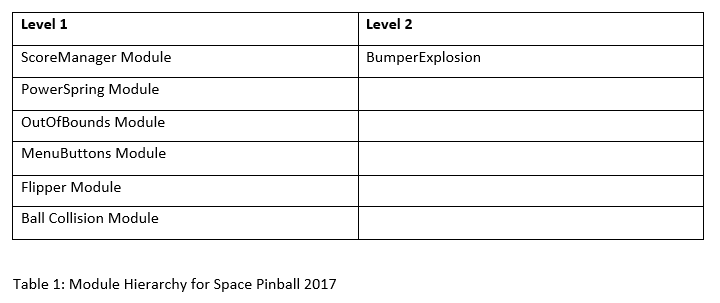
\includegraphics[scale=0.9]{1.png}

\section{Connection Between Requirements and Design} \label{SecConnection}

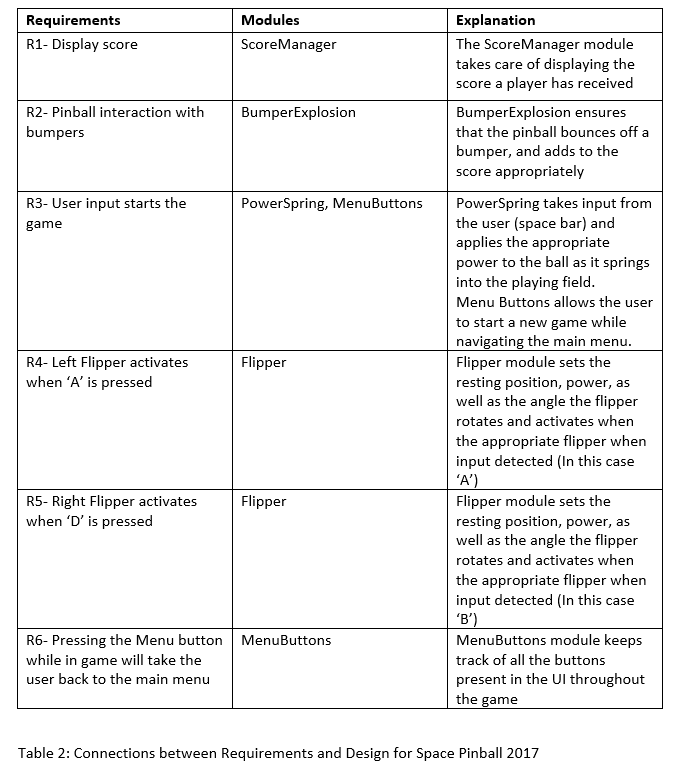
\includegraphics[scale=0.9]{2.png}

\section{Module Decomposition} \label{SecMD}


\section{Traceability Matrix} \label{SecTM}

This section shows two traceability matrices: between the modules and the
requirements and between the modules and the anticipated changes.\\

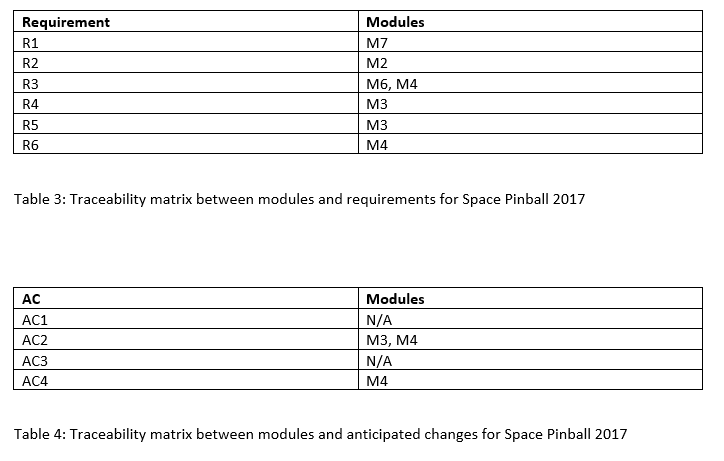
\includegraphics[scale=0.9]{3.png}

\section{Use Hierarchy Between Modules} \label{SecUse}

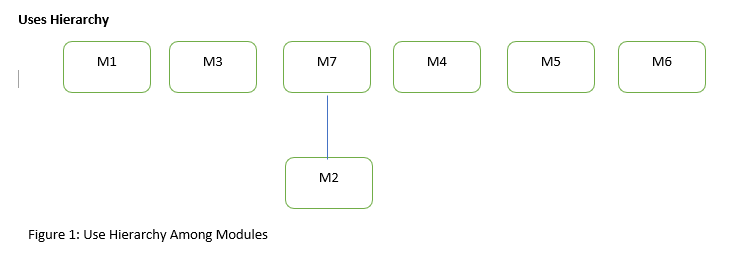
\includegraphics[scale=0.9]{4.png}
\newpage

\section{Gantt Chart}


\begin{figure}[h]
  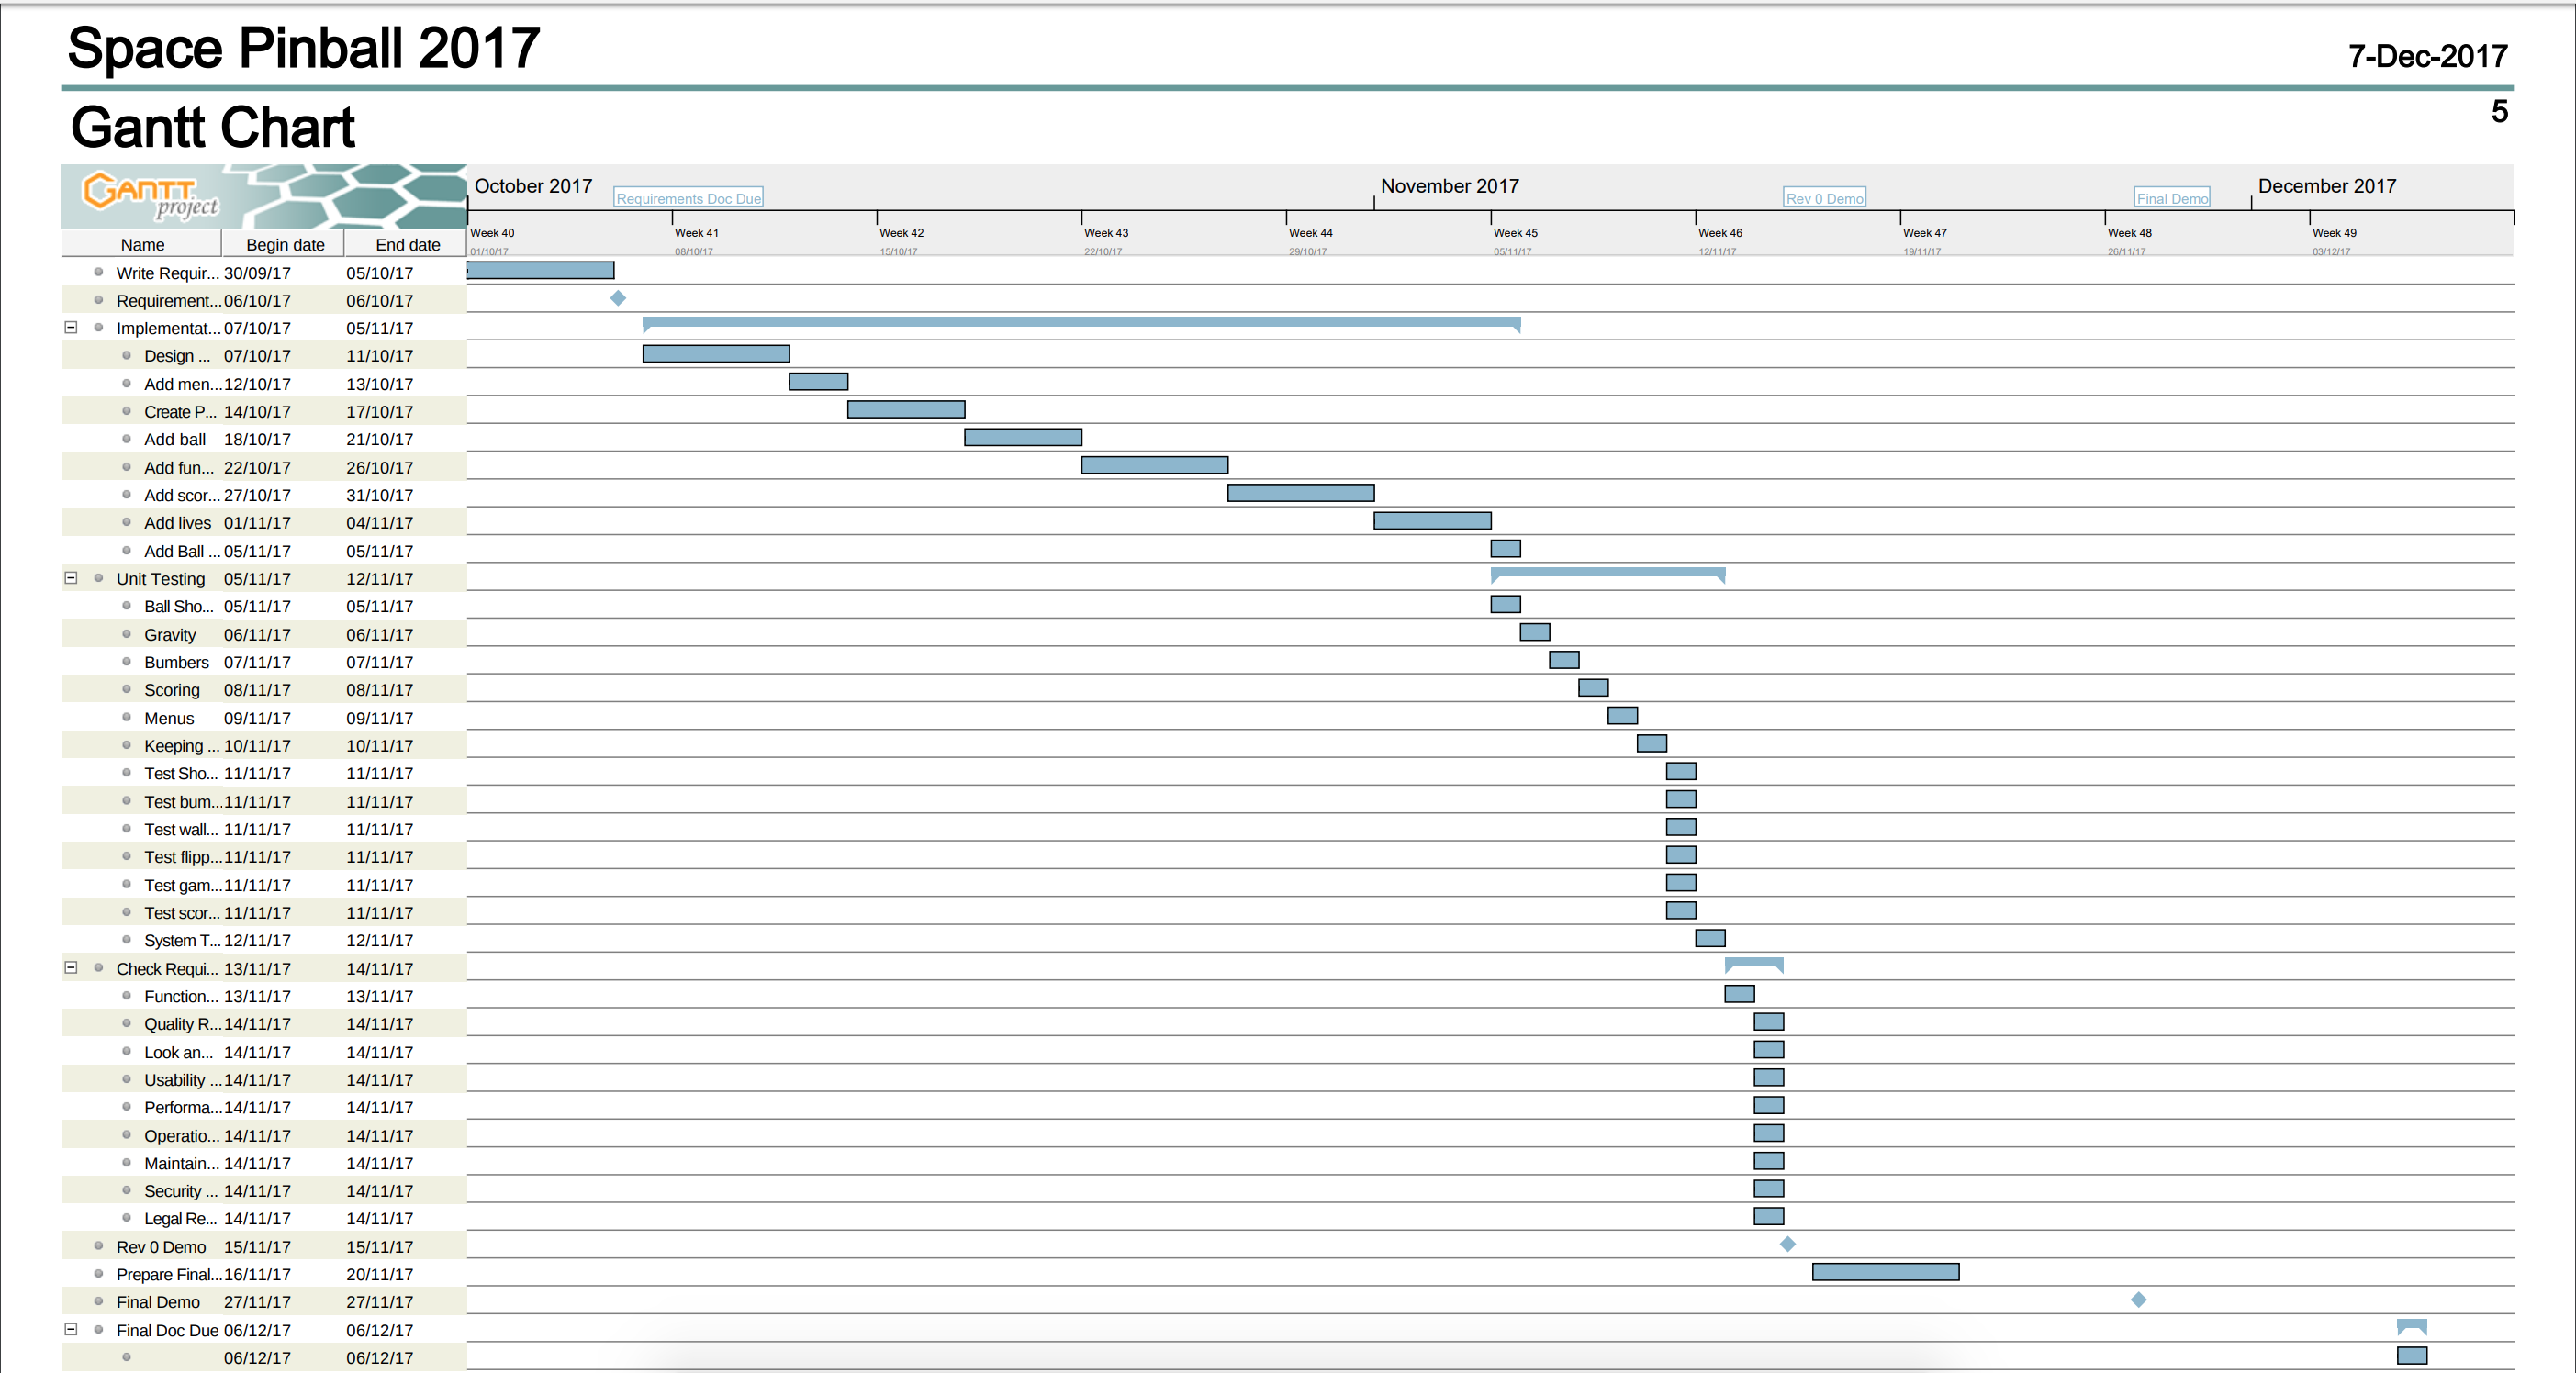
\includegraphics[scale=0.19]{gan.png}
  \caption{Gantt Chart}
  \label{fig:Gantt Chart}
\end{figure}

\begin{figure}[h]
  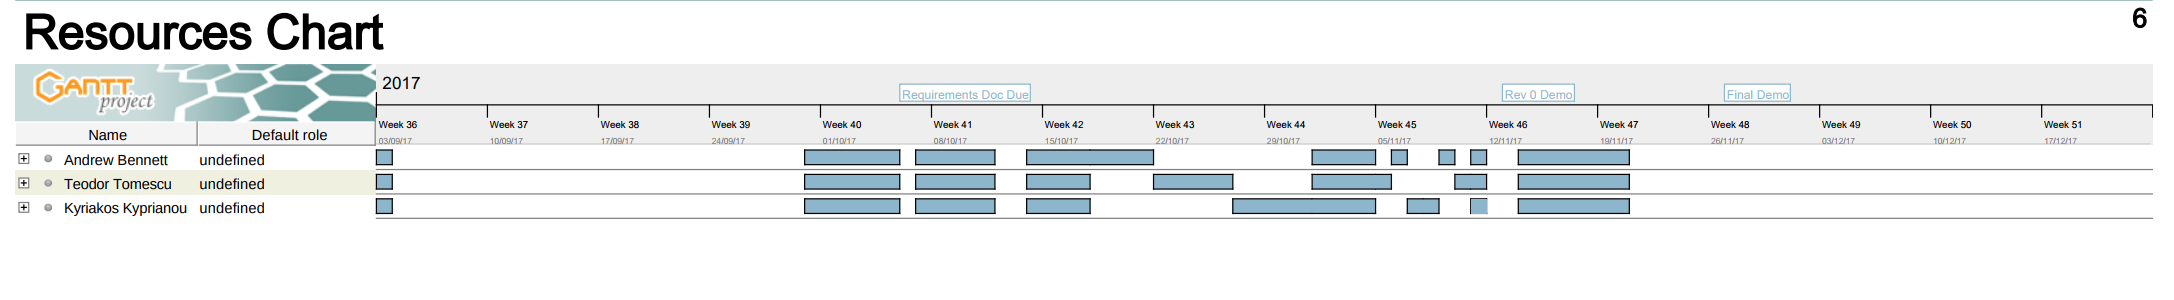
\includegraphics[scale=0.4]{res.png}
  \caption{Resources Chart}
  \label{fig:Resources Chart}
\end{figure}



\clearpage

\end{document}
